% !TEX root = ../notes_missingsemester.tex
% Chapter 5: The Backend — APIs & Services
%%%%%%%%%%%%%%%%%%%%%%%%%%%%%%%%%%%%%%%%%%%%%%%%%%%%%%%%%%%%%%%%%%%%%%

% POST IMPROVEMENTS 2026:
% 1. Add a TikZ figure of the request flow from curl to systemd.
% 2. Provide a pre-baked v0.3 reference repo so catch-up takes a single clone.

\index{API}\index{FastAPI}\index{HTTP}\index{REST}\index{systemd}\index{Pydantic}\index{uvicorn}
\chapter{The Backend: APIs \& Services}
\printchapterversion{05_apis_services}
\newthought{API First. Anyone who doesn't do this, will be fired.}

% ==============================================================================================
% BLOCK 1: INTRODUCTION
% ==============================================================================================

\section{The Why}\index{HTTP}\index{API}

Block~4 left us with \texttt{app/classifier.py}, a function that turns
a 28-by-28 array of pixels into a prediction dictionary.
The function works.
\texttt{predict.py} proves it on real MNIST samples.
What it cannot do is be reached from anywhere except the same Python
process that imported it.

\newthought{This Block}\index{PixelWise}.
is the first that exposes the application to the outside world.
Every client that follows, whether a browser frontend, an automated test
runner, or a monitoring probe, talks to the service through the contract
you design here.

\newthought{HTTP is the protocol} that every browser, every CLI tool,
and every web service in this course speaks.
Figure~\ref{fig:api_flow} shows the path a single request takes through
the stack you will build in this Block.


\begin{figure}
\centering
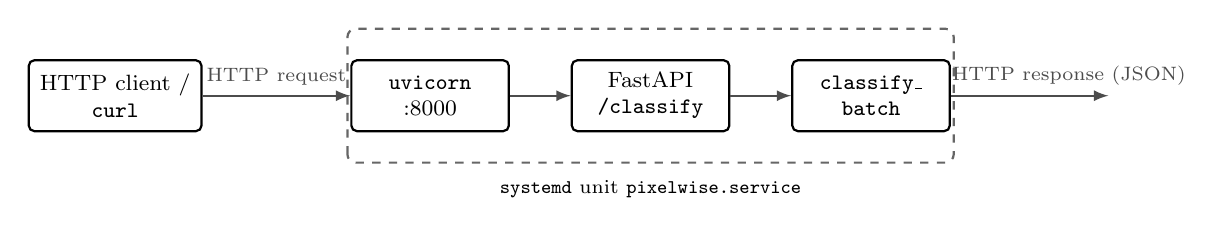
\begin{tikzpicture}[
    every node/.style={font=\footnotesize, align=center},
    box/.style={rectangle, draw=black, thick, rounded corners=2pt, minimum width=2.0cm, minimum height=0.9cm, inner sep=4pt},
    arr/.style={-latex, thick, black!70}
]
\node[box] (cli) at (-1.0, 0) {HTTP client /\\\texttt{curl}};
\node[box] (uv)  at (3.0, 0)  {\texttt{uvicorn}\\:8000};
\node[box] (fa)  at (5.8, 0)  {FastAPI\\\texttt{/classify}};
\node[box] (cf)  at (8.6, 0)  {\texttt{classify\_}\\\texttt{batch}};
\draw[arr] (cli.east) -- node[above]{\scriptsize HTTP request} (uv.west);
\draw[arr] (uv.east)  -- (fa.west);
\draw[arr] (fa.east)  -- (cf.west);
\draw[arr] (cf.east)  -- ++(2.0,0)
    node[above, pos=0.75]{\scriptsize HTTP response (JSON)};
\draw[black!60, thick, dashed, rounded corners=3pt]
    (1.95, -0.85) rectangle (9.65, 0.85);
\node[font=\scriptsize, anchor=north] at (5.8, -0.95)
    {\texttt{systemd} unit \texttt{pixelwise.service}};
\end{tikzpicture}
\caption{\rule{0pt}{1.4cm}\\
Request and response flow for a single classification. The client sends an HTTP request to \texttt{uvicorn}; FastAPI dispatches it to the \texttt{/classify} handler, which calls \texttt{classify\_batch} from Block~4. The dictionary returned by \texttt{classify\_batch} is serialised to JSON and travels back along the same path as the HTTP response. The whole stack runs under a \texttt{systemd} unit that restarts it if it crashes.}
\label{fig:api_flow}
\end{figure}

\newthought{A service} is what \texttt{predict.py} becomes when you wrap
it in HTTP and run it under a supervisor.
\texttt{uvicorn}\index{uvicorn} is the HTTP server that hosts the FastAPI
application; \texttt{systemd}\index{systemd} is the supervisor that
keeps \texttt{uvicorn} running, restarts it when it crashes, and captures
its logs, turning it into someting that survives.



\subsection{Hands On Experience}



\newthought{The contract becomes the product.}
Once the service~\cite{WintersSoftwareEngGoogle2020} is running, the request and response shapes are what
every other component in the system depends on.
Change them silently and the frontend breaks; document them clearly and
new clients can integrate without ever reading your Python.
Ones an API is public, it will be digested, users will build on it, and it will be hard to change~\cite{BrooksMythicalManMonth1995}.



\newthought{This fifth block} introduces the backend service layer for PixelWise.
By the end you will have
\begin{itemize}
    \item understood HTTP and REST well enough to design and probe an endpoint,
    \item written request and response contracts as Pydantic models,
    \item wrapped \texttt{classify\_batch} in a FastAPI application,
    \item added API key authentication and basic rate limiting,
    \item run the service under \texttt{systemd}, observed crashes, and read its logs with \texttt{journalctl}.
\end{itemize}

\marginnote{\newthought{The script-to-service jump.}\index{service}
A script runs once, prints, exits.
A service runs continuously, accepts requests, returns responses, survives
crashes.
The work in this block is what turns the first into the second; the
classifier itself does not change.}



% ==============================================================================================
\newpage
\section{Optional Exercise: Catch Up to \texttt{v0.3}}\index{exercises}\index{Git!tag}\index{recovery}

\marginnote{\newthought{Tag map.}\index{Git!tag}
\texttt{v0.3} marks the end of Block~4, \texttt{v0.4} will mark the end
of this block.
Browse the full set at
\url{https://github.com/schutera/pixelwise/tags}.}

\newthought{Catching up via tag.}\index{Git!tag}\index{recovery}
This catch-up extends the one in Block~4. If you have not done that one,
do it first: It lands you at \texttt{v0.2}, the end-of-Block~3 state. The
exercise here picks up from there and rewinds to \texttt{v0.3}, the
end-of-Block~4 state, with the classifier module in place, the model
artefact pulled into \texttt{models/}, and \texttt{.env} pinned to the
model release.


\newthought{Dev only.} Block~4 deliberately left \texttt{prod} behind:
The classifier had no HTTP entry point, so pulling the code there would
have added an unused \texttt{app/classifier.py} to the production
checkout. This catch-up does the same. Bring \texttt{dev} to \texttt{v0.3}
and leave \texttt{prod} where Block~4 left it; the \texttt{systemd}
exercise later in this block is what finally promotes the service to
\texttt{prod}.

\newthought{Three layers to restore on \texttt{dev}.} Block~4 produced
Git-tracked changes, the new \texttt{app/classifier.py} and
\texttt{predict.py}, an updated \texttt{setup-server.sh}, and a refreshed
\texttt{.env.example}. It also produced unversioned state, the model
artefact \texttt{digit\_classifier\_v1.pkl} in \texttt{models/}, plus
three new \texttt{.env} entries, \texttt{MODEL\_REPO},
\texttt{MODEL\_VERSION}, and \texttt{MODEL\_PATH}. \texttt{git reset
-{}-hard v0.3} restores the first layer,
\texttt{cp .env.example .env} seeds the third, and the extended
\texttt{setup-server.sh} pulls the artefact once \texttt{.env} is in
place.

\newthought{Run the catch-up on \texttt{dev}.}
Rewind the repository to \texttt{v0.3}, refresh \texttt{.env} from the
updated example, run \texttt{setup-server.sh} to pull system packages and
the model artefact, reinstall pinned dependencies if your virtual
environment was wiped, and run \texttt{predict.py} to confirm the
integration works end to end. The exact commands are in the margin.

\marginnote{\newthought{Sequence on \texttt{dev}.}\\[0.4em]
\texttt{cd \textasciitilde/pixelwise}\\
\texttt{git fetch origin -{}-tags}\\
\texttt{git reset -{}-hard v0.3}\\
\texttt{cp .env.example .env}\\
\texttt{bash setup-server.sh}\\
\texttt{source .venv/bin/activate}\\
\texttt{pip install -r requirements.txt}\\
\texttt{python predict.py}\\[0.3em]
If \texttt{.venv/} is missing, run
\texttt{python3 -m venv .venv} before the
\texttt{source} step.}

\marginnote{\newthought{Already have a fork?}\index{Git!fork}
If your own fork carries the \texttt{v0.3} tag, swap \texttt{origin} on
\texttt{dev} with
\texttt{git remote set-url origin git@github.com:<you>/pixelwise.git}
so push and pull continue to target your account.
The HTTPS clone on \texttt{prod} stays read-only.}

\newthought{You are now} at the state where Block~4 ended:
\texttt{dev} is at \texttt{v0.3} and \texttt{prod} still trails behind,
ready to start Block~5.



% ==============================================================================================
% BLOCK 2: CONCEPTS AND PRACTICE
% ==============================================================================================

\newpage
\section{HTTP and REST}\index{HTTP}\index{REST}

\marginnote{\newthought{HTTP}\index{HTTP} is the request and response
protocol that sits underneath every browser call, every \texttt{curl}
invocation, and every API in this course.
A reference overview of the methods, status codes, and headers lives
\href{https://developer.mozilla.org/en-US/docs/Web/HTTP}{here}.}

\newthought{Every web interaction is a request and a response.}
The client sends a request that names a method, a path, and an optional
body; the server sends back a status code, headers, and an optional body.
The protocol carries no state of its own: each request is interpretable on
its own, without knowledge of any previous request from the same client.

\marginnote{\newthought{Status codes you will see most.}\index{HTTP!status codes}
Three-digit numbers grouped by leading digit. \texttt{2xx} means success,
\texttt{4xx} means the client made a mistake, \texttt{5xx} means the
server made a mistake.
\begin{itemize}
    \item \texttt{200} OK,
    \item \texttt{201} Created,
    \item \texttt{400} Bad Request,
    \item \texttt{401} Unauthorized,
    \item \texttt{404} Not Found,
    \item \texttt{422} Unprocessable Entity,
    \item \texttt{429} Too Many Requests,
    \item \texttt{500} Internal Server Error.
\end{itemize}}

\newthought{Methods and Queries you will use.}\index{HTTP!methods}
\begin{itemize}
    \item \texttt{GET} retrieves,
    \item \texttt{POST} submits,
    \item \texttt{PUT} replaces,
    \item \texttt{DELETE} removes.
\end{itemize}
PixelWise uses \texttt{POST} for \texttt{/classify} when the client
submits a drawing, and \texttt{GET} for \texttt{/results} and
\texttt{/health} when the client reads state.

\marginnote{\newthought{Stateless}\index{stateless} is the load-bearing
property of HTTP.
The server keeps no per-client memory between requests; everything the
server needs to act is in the current request, including any authentication
token.
This is what lets you scale.}

\marginnote{\newthought{REST}\index{REST} is the architectural style that
maps the HTTP verbs onto application resources.
Each resource has a stable URL; each verb has a clear meaning.
We use REST because it is the convention every frontend, every tool, and
every framework in this stack expects, not because it is the only valid
choice.
A reference introduction to the style and its conventions lives
\href{https://developer.mozilla.org/en-US/docs/Glossary/REST}{here}.}

\newthought{REST principles} layer convention on top of the protocol.
Every distinct thing the API exposes is a resource with a stable URL:
\texttt{/classify}, \texttt{/results}, \texttt{/health}.
Methods do what their names suggest.
Responses are JSON.
Two clients written by two teams, six months apart, agree on what the API
does without ever speaking, because the conventions remove ambiguity.

\marginnote{HTTP status codes reference: \\
\url{https://developer.mozilla.org/en-US/docs/Web/HTTP/Status}\\
REST overview: \\
\url{https://restfulapi.net/}}

\newthought{The interactive definition of an API} is the documentation that
ships with the running service.
FastAPI generates an OpenAPI\index{OpenAPI} specification from your code,
exposes the raw JSON at \texttt{/openapi.json}, and renders it through two
built-in interfaces: Swagger UI\index{Swagger UI} at \texttt{/docs} and
ReDoc\index{ReDoc} at \texttt{/redoc}. Exposing them changes the social
contract: A teammate does not need to read your source to integrate, it's your responsibility to fulfill the stated contract.
Block~3's \texttt{DEBUG=true} flag controls whether the documentation
endpoints are exposed, so the same service is self-documenting in
development and silent in production.

\marginnote{\newthought{One spec, many renderers.}\index{OpenAPI}
\texttt{/openapi.json} is the contract; Swagger UI and ReDoc are two ways
to look at it.
The same spec format is what Flask, Django, Express, and Spring all emit,
and the same renderers and SDK generators work against any of them.\\
OpenAPI: \url{https://www.openapis.org/}\\
Swagger Editor: \url{https://editor.swagger.io/}}



% ==============================================================================================
\newpage
\section{Exercise: HTTP, REST, and \texttt{curl}}\index{exercises}

\newthought{Probe a public API} before writing your own.
\texttt{httpbin.org}\index{httpbin} is a free request-and-response echo
service: It returns a JSON document describing exactly what it just
received, so you can read status codes, headers, and the body of your own
request side by side with the response. On \texttt{dev}, with the virtual
environment active:

\begin{verbatim}
curl -i https://httpbin.org/get
curl -i -X POST https://httpbin.org/post \
    -H "Content-Type: application/json" \
    -d '{"hello": "world"}'
\end{verbatim}

\marginnote{\newthought{Read each section of the response.}
\texttt{HTTP/2 200} is the status line.
The lines that follow are headers; the blank line marks the boundary; the
JSON below it is the body.
Every HTTP response in this course has the same shape.}

\marginnote{\newthought{JSON Syntax}\index{JSON}
Objects \texttt{\{\dots\}}, arrays \texttt{[\dots]}, strings in double
quotes, numbers and booleans and \texttt{null} unquoted, commas between
items but never trailing.
Spec: \url{https://www.json.org/}}

\newthought{The body is JSON.}\index{JSON}
JSON is the universal serialisation format for web APIs: A text-shaped
tree of objects, arrays, strings, numbers, booleans, and \texttt{null}.
Your \texttt{GET} response body is short enough to read in full:

\begin{verbatim}
{
  "args": {},
  "headers": {
    "Accept": "*/*",
    "Host": "httpbin.org",
    "User-Agent": "curl/7.81.0"
  },
  "origin": "203.0.113.42",
  "url": "https://httpbin.org/get"
}
\end{verbatim}

Curly braces enclose an object, each key is a quoted string, and each
value is a primitive, an array, or another object. PixelWise's
\texttt{/classify} response will use the same shape, with keys
\texttt{prediction}, \texttt{confidence}, and \texttt{scores}, parsed
identically by any client in any language.

\marginnote{\newthought{Answers.}\index{HTTP!methods}
\texttt{POST /classify}: Image data does not fit in a query string;
\texttt{POST} carries it in the body and is not cached. \texttt{200 OK}
with the prediction.\\[2pt]
\texttt{GET /results}: Safely cacheable, no side effect.
\texttt{200 OK}.\\[2pt]
\texttt{GET /health}: Reads liveness, no side effect. \texttt{200 OK},
or \texttt{503 Service Unavailable} when unhealthy.}

\newthought{Pick the verb} for each PixelWise endpoint and say what
success looks like:
\begin{itemize}
    \item \texttt{/classify}: Submit a drawing for prediction.
    \item \texttt{/results}: Read the last 10 predictions.
    \item \texttt{/health}: Check whether the service is alive.
\end{itemize}






% ==============================================================================================
\newpage
\section{FastAPI in Practice}\index{FastAPI}\index{path operation}

\newthought{FastAPI is a modern Python web framework} built on top of
Pydantic and the ASGI standard.
It generates interactive API documentation automatically, validates inputs
and outputs against the models you declared, and runs on \texttt{uvicorn}, an
asynchronous HTTP server fast enough that your bottleneck will be the model,
not the framework.

\newthought{Pydantic.}\index{Pydantic}
Python data-validation library. A class inherits from \texttt{BaseModel}
and declares typed fields; Pydantic validates incoming data against the
schema and raises a structured error on mismatch. FastAPI runs the same
check at the HTTP boundary and returns
\texttt{422 Unprocessable Entity} on failure.\\
\url{https://docs.pydantic.dev/}

\marginnote{FastAPI: \url{https://fastapi.tiangolo.com/}\\
Pydantic: \url{https://docs.pydantic.dev/}\\
uvicorn: \url{https://www.uvicorn.org/}\\
ASGI: \url{https://asgi.readthedocs.io/}}

\newthought{A path operation} is the unit of routing in FastAPI: A
Python function whose decorator binds it to one HTTP method and one URL
path. When the application starts, FastAPI walks the decorated functions
and builds a routing table that \texttt{uvicorn} consults on every
incoming request. The type hints on the parameters are not just
documentation: They are read at registration time and turned into a
validator that runs before your function body executes. A request that
fails the validator never reaches your code. It is rejected at the
boundary with a \texttt{422} response whose body lists exactly which
field was wrong and why, so the caller can fix the request without
guessing at your implementation.

\newthought{The decorator is the contract.}
\texttt{@app.post("/classify", response\_model=Classify\-Response)}
encodes three things at once: The method clients must use, the path they
must hit, and the schema the response must satisfy. The first two shape
the routing table. The third shapes what leaves the server. FastAPI runs
the value your function returns through \texttt{ClassifyResponse} on the
way out, drops fields that are not declared on the model so internal
state cannot leak by accident, and fills the OpenAPI schema served at
\texttt{/docs} from the same class. A handler that returns the wrong
shape fails inside the framework on the first request, long before a
downstream client notices that the documented contract has drifted from
the implementation.

\newthought{\texttt{curl} is a command-line HTTP client.}\index{curl}
It writes the bytes of a request directly to a socket and prints the
bytes of the response, with no browser, no JavaScript, and no implicit
defaults beyond what you pass on the command line. That is what makes it
useful for debugging: The request you send is exactly the request you
typed, so the only place a bug can hide is in your invocation or in the
server. The interactive \texttt{/docs} page, by contrast, does a lot on
your behalf. It JSON-encodes the body for you, sets the
\texttt{Content-\linebreak[1]Type: application/json} header on every
\texttt{POST}, and, once you click \texttt{Authorize}, attaches the API
key header to subsequent calls. A request that succeeds from
\texttt{/docs} and fails from \texttt{curl} therefore points at
something the form was adding silently, almost always a header you
forgot on the command line. A request that fails from both rules out
the client and points back at the handler. The exercise below gives the
exact \texttt{curl} invocations against the running service so you can
compare the two side by side.

\marginnote{curl: \url{https://curl.se/}\\
\texttt{-X} sets the HTTP method.\\
\texttt{-H} sets a header.\\
\texttt{-d} sets the request body.\\
\texttt{-i} prints the response headers alongside the body, useful when a
status code surprises you.}

\newthought{Three endpoints} cover the surface this block exposes:
\texttt{POST /classify} performs inference, \texttt{GET /results} is a stub
that a later persistence layer will fill in, and \texttt{GET /health}
reports liveness so a monitor can tell whether the service is up.



% ==============================================================================================
\newpage
\section{Exercise: Building \texttt{app/main.py}}\index{exercises}

\newthought{Install the runtime dependencies} into the dev virtual
environment and pin them:

\marginnote{\newthought{The \texttt{[standard]} extra} on \texttt{uvicorn}
pulls in optional but recommended packages that ship alongside the core
server: \texttt{httptools} for a faster HTTP parser, \texttt{uvloop} for
a faster event loop on Linux, \texttt{websockets} for the WebSocket
protocol, and \texttt{watchfiles} so \texttt{--reload} can detect code
changes during development. Without the extra you still get a working
server, just slower and without auto-reload.}

\begin{verbatim}
source .venv/bin/activate
pip install fastapi uvicorn[standard] \
    slowapi pydantic
pip freeze > requirements.txt
\end{verbatim}

\marginnote{\newthought{Ctrl\,+\,R in the terminal} starts a reverse
search through your shell history. Hit it, type a few characters of a
command you ran earlier, such as \texttt{pip freeze}, and the most
recent match appears. Press Ctrl\,+\,R again to step further back, Enter
to run the match, or the right arrow to edit it before running. This is
much faster than retyping or looking up commands again or scrolling with the up arrow.}

\newthought{Wire the path operations from the theory above into a working
service.}
Open \texttt{app/main.py} in nano and write the request and response
models followed by the three endpoints:

\begin{verbatim}
from fastapi import FastAPI
from pydantic import BaseModel
import numpy as np
from app.classifier import classify_batch

class ClassifyRequest(BaseModel):
    pixels: list[list[int]]

class ClassifyResponse(BaseModel):
    prediction: str
    confidence: float
    scores: dict[str, float]

app = FastAPI()

@app.get("/health")
def health():
    return {"status": "ok", "model_version": "v1"}

@app.get("/results")
def results():
    return {"results": [],
            "note": "persistence not yet implemented"}

@app.post("/classify",
          response_model=ClassifyResponse)
def classify(req: ClassifyRequest):
    arr = np.array(req.pixels,
                   dtype=np.uint8)[np.newaxis]
    return classify_batch(arr)[0]
\end{verbatim}

\marginnote{\newthought{The shape lives in two places now.}\index{contract}
\texttt{ClassifyResponse} in Python and the dictionary
\texttt{classify\_batch} returns from Block~4.
A field named \texttt{prediction} in one and \texttt{predicted} in the
other is exactly the kind of mismatch the contract is supposed to
prevent; keeping them aligned is part of the work.}

\marginnote{\newthought{Run it locally:}\index{uvicorn}
\texttt{uvicorn app.main:app --reload --port 8000}.
The \texttt{--reload} flag restarts on every code change, which is what you
want in development and never want in production.
Open \url{http://localhost:8000/docs} to see the auto-generated OpenAPI
page; click ``Try it out'' on \texttt{POST /classify} to issue a real
request without leaving the browser.}

\newthought{Test with curl from another terminal:}

\begin{verbatim}
curl http://localhost:8000/health
curl -X POST http://localhost:8000/classify \
  -H "Content-Type: application/json" \
  -d '{"pixels": [[0,0,...], ...]}'
\end{verbatim}

A 28-by-28 zero array returns a low-confidence prediction; a real digit
loaded from MNIST returns the right answer.
The first end-to-end loop is when this works.

\marginnote{\newthought{Send a deliberately wrong shape.}\index{HTTP!422}
Submit a 27-by-27 grid and read the 422 response.
Pydantic rejects the request before the handler runs, with a structured
error that tells the client exactly which field was wrong.
This is the input validation boundary doing its job.}



% ==============================================================================================
\newpage
\section{Authentication and Rate Limiting}\index{authentication}\index{rate limiting}

\newthought{Even a classroom service needs both.}
30 students hitting the same endpoint in the same minute is enough load
to surface a rate-limit problem on the first day.
A leaking debug build is enough to see the API key reach a place it does
not belong.
Authentication and rate limiting are layered defences: the first answers
``who is calling'', the second answers ``how often''.

\newthought{API key authentication} is the simplest form that fits this
course. The client sends a secret in a header; the server compares it to
the value in \texttt{.env} and rejects requests that do not match with
\texttt{401 Unauthorized}. FastAPI exposes the header through a small
dependency function that runs before every protected handler, which the
exercise wires up.

\marginnote{\newthought{Why a header?}\index{HTTP!headers}
Headers travel separately from the body and the URL, so the secret never
ends up in the path component of an access log.
Putting the key in a query parameter would write it into every log line
the request touched on the way to the server.}

\newthought{Rate limiting} prevents both abuse and accident.
\texttt{slowapi} attaches a per-route decorator that counts requests per
client IP and rejects them with HTTP \texttt{429} when the limit is
exceeded. A budget like ``30 requests per minute per IP'' is enough to
stop a runaway client without inconveniencing a normal one.

\marginnote{\newthought{Where does rate limiting belong?}\index{slowapi}
Application-level limits are easy to write and travel with the code.
Reverse-proxy limits, a topic we will revisit later in the course, run in
front of the application and protect it even when it is overwhelmed.
Both layers are useful; the latter is harder to bypass.\\
slowapi: \url{https://github.com/laurentS/slowapi}}

\newthought{Pydantic, the API key middleware, and the rate limiter}
together form a three-stage filter at the boundary of the application.
A request that arrives must parse as JSON, match the schema, present a
valid key, and stay within the rate budget before any inference code runs.
Each stage rejects with a different status code, so a client failure tells
you exactly which contract was violated.



% ==============================================================================================
\newpage
\section{Exercise: API Key Auth and Rate Limiting}\index{exercises}

\newthought{Add the defensive layer from the theory above to the service.}
Add API key middleware to \texttt{app/main.py}:

\begin{verbatim}
from fastapi import Header, HTTPException, Depends
import os

def verify_api_key(x_api_key: str = Header(...)):
    if x_api_key != os.getenv("SECRET_API_KEY"):
        raise HTTPException(
            status_code=401, detail="Invalid API key")

@app.post("/classify",
          response_model=ClassifyResponse,
          dependencies=[Depends(verify_api_key)])
def classify(req: ClassifyRequest):
    ...
\end{verbatim}

\marginnote{\newthought{The header travels in every request.}\index{X-API-Key}
\texttt{X-API-Key} is a custom header name; FastAPI's \texttt{Header(...)}
maps it to the function parameter automatically.
A missing header returns 422 (Pydantic-level), a wrong value returns 401
(your handler).}

\newthought{Add rate limiting} with \texttt{slowapi}:

\begin{verbatim}
from slowapi import Limiter
from slowapi.util import get_remote_address
from slowapi.middleware import SlowAPIMiddleware

limiter = Limiter(key_func=get_remote_address)
app.state.limiter = limiter
app.add_middleware(SlowAPIMiddleware)

@app.post("/classify")
@limiter.limit("30/minute")
def classify(req: ClassifyRequest):
    ...
\end{verbatim}

\newthought{Test all three failure modes:}
\begin{itemize}
    \item Missing header: 422.
    \item Wrong key: 401.
    \item More than 30 requests in a minute: 429.
\end{itemize}
Each one should reach \texttt{curl} as a status code rather than as a
crash; that is the entire point of the boundary.

\marginnote{\newthought{Watch a 429 happen.}\index{HTTP!429}
A small Bash loop firing 40 \texttt{curl} requests at the endpoint inside
the same minute should see the last ten return \texttt{429 Too Many
Requests}.
The remaining requests stay rejected until the window rolls over.}



% ==============================================================================================
\newpage
\section{From Dev to Production: \texttt{systemd}}\index{systemd}\index{systemctl}\index{journalctl}

\newthought{\texttt{uvicorn} runs fine for testing,}\index{uvicorn}
but one Ctrl+C and it is gone.
A closed terminal kills it.
A reboot kills it.
A panic in a worker kills it without restart.
None of that is the behaviour of a service.

\marginnote{\newthought{Why \texttt{systemd}?}\index{systemd}
Running \texttt{uvicorn} in a terminal works until you close the terminal.
Running it under \texttt{systemd} survives reboots, restarts on crash,
and writes its output to a structured log you can query later.
The classroom requirement and the production requirement are the same.}

\newthought{\texttt{systemd}} is the OS-level supervisor that comes with
Ubuntu. It starts services on boot, restarts them when they crash,
captures their output to a structured log, and exposes a uniform
interface for operators. The contract between you and \texttt{systemd}
is a unit file, an INI-style description with three sections: An
\texttt{[Unit]} block for metadata and dependencies, a \texttt{[Service]}
block naming the user, working directory, environment file, command to
run, and restart policy, and an \texttt{[Install]} block declaring when
the unit should be started. The exercise below has the full file
PixelWise needs.

\marginnote{\newthought{We use a fraction} of what \texttt{systemd} can do.
It also manages timers (cron with dependency awareness), socket activation
(start on connection), resource limits (cap CPU/memory per service), and
dependency ordering (start the database before the app).
It is the init system of virtually every modern Linux server.\\
systemd: \url{https://www.freedesktop.org/wiki/Software/systemd/}}

\newthought{\texttt{systemctl}}\index{systemctl} is the operator's interface
to \texttt{systemd}. \texttt{start}, \texttt{stop}, and \texttt{restart}
are the verbs you reach for during deployment; \texttt{status} reports
the current state and the last few lines of output; \texttt{enable} marks
the service as one that should start on boot;
\texttt{daemon-reload} tells \texttt{systemd} to re-read its unit files
after you edit one. The exercise runs the full sequence on \texttt{prod}.

\marginnote{\newthought{\texttt{journalctl}}\index{journalctl} is where you
go first when something breaks.
\texttt{journalctl -u pixelwise} prints every log line from your service
since boot; \texttt{-f} follows new lines as they arrive, the way
\texttt{tail -f} follows a file; \texttt{--since "5 min ago"} narrows the
window when the bug is recent.}

\newthought{In production} you would run \texttt{gunicorn}\index{gunicorn}
in front of \texttt{uvicorn} to spawn multiple worker processes, giving
you concurrency and crash isolation.
For our classroom setup, a single \texttt{uvicorn} worker behind
\texttt{systemd} is sufficient.
\texttt{gunicorn} is standard in production Python deployments; students
who deploy beyond this course will encounter it within the first week.



% ==============================================================================================
\newpage
\section{Exercise: Running as a \texttt{systemd} Service}\index{exercises}

\newthought{Promote the service from a foreground \texttt{uvicorn} to a
supervised \texttt{systemd} unit.}
Push your code to GitHub from \texttt{dev}, then SSH into the server and
pull:

\begin{verbatim}
# on dev
git add app/main.py requirements.txt .env.example
git commit -m "Add FastAPI service with auth and limits"
git push

# on prod
ssh produser@192.168.56.11
cd /opt/pixelwise
git pull
source .venv/bin/activate
pip install -r requirements.txt
\end{verbatim}

\newthought{Create the unit file} at
\texttt{/etc/systemd/system/pixelwise.service} on \texttt{prod}.
Open it in nano:

\begin{verbatim}
sudo nano /etc/systemd/system/pixelwise.service
\end{verbatim}

Paste the following, save with \texttt{Ctrl+O}, exit with \texttt{Ctrl+X}:

\begin{verbatim}
# /etc/systemd/system/pixelwise.service
[Unit]
Description=PixelWise API
After=network.target

[Service]
User=produser
WorkingDirectory=/opt/pixelwise
EnvironmentFile=/opt/pixelwise/.env
ExecStart=/opt/pixelwise/.venv/bin/uvicorn \
    app.main:app --host 0.0.0.0 --port 8000
Restart=always
RestartSec=3

[Install]
WantedBy=multi-user.target
\end{verbatim}

Then reload \texttt{systemd}, enable the unit so it survives reboots,
and start it:

\begin{verbatim}
sudo systemctl daemon-reload
sudo systemctl enable pixelwise
sudo systemctl start pixelwise
sudo systemctl status pixelwise
\end{verbatim}

\marginnote{\newthought{Read the status output.}\index{systemctl}
\texttt{Active: active (running)} is what you want.
\texttt{Active: failed} means the unit started and exited; the last few
log lines below the status block usually say why.
\texttt{Active: inactive (dead)} means the unit was never started.}

\newthought{Kill it on purpose.}
A service that has never crashed is a service whose recovery has never been
tested.

\begin{verbatim}
sudo systemctl stop pixelwise
sudo systemctl status pixelwise
sudo systemctl start pixelwise
journalctl -u pixelwise --since "5 min ago"
\end{verbatim}

\marginnote{\newthought{First end-to-end loop on the network.}\index{curl}
From \texttt{dev}: \\
\texttt{curl -X POST http://192.168.56.11:8000/classify
-H "X-API-Key: ..." -d '\{...\}'}.
A live prediction from the server, served by \texttt{systemd}-supervised
\texttt{uvicorn}, returns to your terminal on \texttt{dev}.
The system is reachable across machines for the first time.}

\newthought{A note on what comes next.}
The service runs, the contract is documented, the supervisor restarts
crashes; what is missing is memory.
\texttt{GET /results} returns an empty list because nothing is being stored.
Persistence is a thread we will pick up later in the course, when every
prediction becomes a row that survives the response.



% ==============================================================================================
\newpage
\section{Optional Exercise: Inspect an OpenAPI Spec}\index{exercises}\index{OpenAPI}\index{Swagger UI}

\newthought{The renderer is interchangeable.}\index{OpenAPI}
Once a service exposes \texttt{/openapi.json}, any tool that speaks
OpenAPI can render it, generate a client for it, or run contract tests
against it. This exercise is a short tour of that ecosystem; it adds no
code to PixelWise, only confidence that the contract is portable. Come
back to it once your own service is up and rerun the same steps against
\texttt{http://localhost:8000/openapi.json}.

\newthought{Pull the raw spec} from a public OpenAPI service, since
PixelWise has not been wrapped in FastAPI yet:

\begin{verbatim}
curl -s https://petstore3.swagger.io/api/v3/openapi.json \
    | head -40
\end{verbatim}

The top of the document lists \texttt{openapi}, \texttt{info},
\texttt{servers}, and \texttt{paths}. Every FastAPI service you build
will emit a document with the same top-level keys.

\newthought{Open the spec in another renderer.}\index{Swagger Editor}
Visit \url{https://editor.swagger.io/}, choose \texttt{File} and then
\texttt{Import URL}, and paste
\texttt{https://petstore3.swagger.io/api/v3/openapi.json}. The same
contract now appears in a different UI from the one served by
\texttt{/docs}, with the same endpoints, the same models, and the same
example payloads. The renderer is interchangeable.

\marginnote{\newthought{Why this matters.}\index{API contract}
A frontend team consuming your API rarely opens your Python.
They open the OpenAPI spec, generate a typed client from it, and call
that client from their codebase. The discipline of writing correct
Pydantic models in this block is what makes the generated client correct
on the other side.}

\newthought{Generate a client SDK.}\index{OpenAPI Generator}
\texttt{openapi-python-client} produces a typed Python client from any
OpenAPI spec. On dev, with the virtual environment active:

\begin{verbatim}
pip install openapi-python-client
openapi-python-client generate \
    --url https://petstore3.swagger.io/api/v3/openapi.json
ls
\end{verbatim}

The generated package contains a typed client for every endpoint the
spec declares. The same generator project has back-ends for TypeScript,
Go, Java, and a dozen other languages: One spec, many clients.


% ==============================================================================================
% BLOCK 3: CONSOLIDATION
% ==============================================================================================

\newpage
\section{Self-Reflection and Recap}\index{reflection}\index{recap}

\newthought{Self-Reflection} questions to guide your thoughts during and after the exercises:
\begin{itemize}
    \item What is the difference between running \texttt{uvicorn} manually and running it under \texttt{systemd}?
    \item Why does Pydantic validation matter for security as well as correctness?
    \item What happens when the \texttt{systemd} service crashes, and how does \texttt{Restart=always} help?
    \item Why is \texttt{GET /results} a stub right now, and what would have to arrive to fill it in?
    \item How would you debug a failing endpoint using only \texttt{journalctl}?
    \item Which of the three rejection points (Pydantic, API key, rate limiter) is hardest to bypass, and why?
\end{itemize}

\newthought{Recap} of key concepts:
\begin{itemize}
    \item HTTP is a stateless request-response protocol; REST layers conventions on top so APIs are predictable across teams.
    \item Pydantic models are the API contract; FastAPI enforces them at the boundary and renders them as live documentation.
    \item \texttt{POST /classify}, \texttt{GET /results}, \texttt{GET /health} cover the surface this block exposes; \texttt{/results} is a deliberate stub awaiting a persistence layer.
    \item API keys answer ``who is calling''; rate limits answer ``how often''.
    \item \texttt{systemd} turns a script into a service: starts on boot, restarts on crash, logs to \texttt{journalctl}.
\end{itemize}

\marginnote{\newthought{Security thread.}\index{security}
The API key lives in \texttt{.env}, never in code.
Pydantic models are the input validation boundary; rate limits cap any single
caller; the \texttt{X-API-Key} header keeps the secret out of access logs.
Transport-layer encryption is a thread we will revisit later in the course.}

\marginnote{\newthought{Teaser.} Where do all those predictions go once the
response has been sent?}

\newthought{Milestone.} PixelWise runs as a managed \texttt{systemd}
service on the \texttt{prod} VM.
\texttt{POST /classify} returns live digit predictions; \texttt{GET /results}
is stubbed pending persistence; \texttt{GET /health} reports liveness.
You have killed and restarted the backend at least once and read the logs
with \texttt{journalctl}.
The contract is now the load-bearing surface of the system: every
component that follows will speak to PixelWise through it.
